
% JDR: I spend two full lectures on this.

\usetikzlibrary{decorations.pathreplacing,decorations.markings,angles}

\titleframe{Section 5.5}{Complex Eigenvalues}


%%%%%%%%%%%%%%%%%%%%%%%%%%%%%%%%%%%%%%%%%%%%%%%%%%%%%%%%%%%%%%%%%%%

\begin{frame}
\frametitle{A Matrix with No Eigenvectors}

In recitation you discussed the linear transformation for rotation by $\pi/4$ in
the plane.  The matrix is:
\pause
\[ A = \frac 1{\sqrt 2}\mat{1 -1; 1 1}. \]
\pause
This matrix has no eigenvectors, as you can see geometrically:
\def\theo{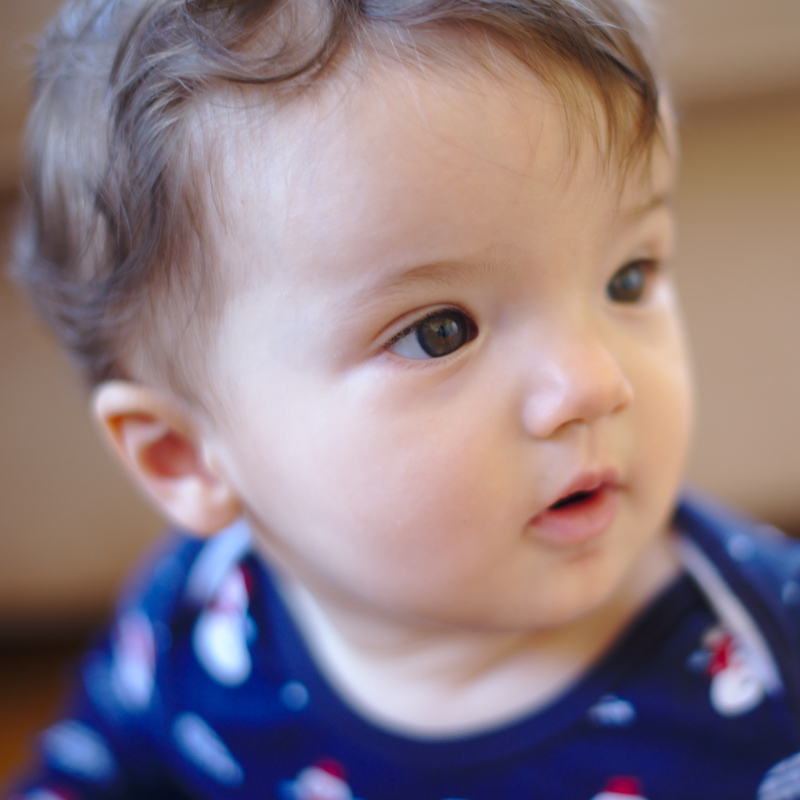
\includegraphics[width=3cm]{figures/theo6.jpg}}\\[1mm]
\hfill
\begin{tikzpicture}
  \begin{scope}
    \clip (0,0) circle[radius=1.5cm];
    \node[circle, thin border] (theo1) at (0,0) {\theo};
  \end{scope}
  \draw[->,opacity=.6] (-1.8,0) -- (1.8,0);
  \draw[->,opacity=.6] (0,-1.8) -- (0,1.8);

  \begin{scope}[xshift=7cm]
  \begin{scope}[rotate=45]
    \clip (0,0) circle[radius=1.5cm];
    \node[transform shape, circle, thin border] 
      (theo2) at (0,0) {\theo};
  \end{scope}
  \draw[->,opacity=.6] (-1.8,0) -- (1.8,0);
  \draw[->,opacity=.6] (0,-1.8) -- (0,1.8);
  \end{scope}

  \draw[->] ($(theo1.east)+(0,.3)$) to[bend left]
    node[midway,above] {$A$}
    node[midway,below=5mm,text width=3cm,align=center] 
      {no nonzero vector $x$ is collinear with $Ax$}
    ($(theo2.north west)+(0,.3)$);

\end{tikzpicture}
\hfill\null

\pause
or algebraically:
\[ f(\lambda) = \lambda^2 - \Tr(A)\,\lambda + \det(A)
= \lambda^2 - \sqrt 2\,\lambda + 1\pause
\implies \lambda = \frac{\sqrt 2\pm\sqrt{-2}}2. \]

\end{frame}


%%%%%%%%%%%%%%%%%%%%%%%%%%%%%%%%%%%%%%%%%%%%%%%%%%%%%%%%%%%%%%%%%%%

\begin{frame}
\frametitle{Complex Numbers}

It makes us sad that $-1$ has no square root.
\pause
If it did, then $\sqrt{-2} = \sqrt{2}\cdot\sqrt{-1}$.

\pause\medskip
\alert{Mathematician's solution:} we're just not using enough numbers!
\pause
We're going to declare by \emph{fiat} that there exists a square root of $-1$.

\pause
\begin{defn}
  The number $i$ is defined such that $i^2 = -1$.
\end{defn}

\pause
Once we have $i$, we have to allow numbers like $a+bi$ for real numbers $a,b$.

\pause
\begin{defn}
  A \emph{complex number} is a number of the form $a+bi$ for $a,b$ in $\R$.
  The set of all complex numbers is denoted $\C$.
\end{defn}

\pause\medskip
Note $\R$ is contained in $\C$: they're the numbers $a + 0i$.

\pause\medskip
We can identify $\C$ with $\R^2$ by $a+bi \ToT {a\choose b}$.
\pause
So when we draw a picture of $\C$, we draw the plane:\\
\hfill
\begin{tikzpicture}[scale=.5, whitebg nodes, thin border nodes]
  \draw[grid lines] (-2,-2) grid (2,2);
  \draw[thick, ->] (-2,0) -- (2,0);
  \draw[<-, overlay] (-2.05,0) -- (-2.5,0) node[left] {real axis};
  \draw[thick, ->] (0,-2) -- (0,2);
  \draw[<-, overlay] (-.05,-1.5) -- ++(-2.5,0) node[left] {imaginary axis};
  \point["$1$" above] at (1,0);
  \point["$i$" left] at (0,1);
  \point at (0,0);
  \point["$1-i$" below] at (1,-1);
\end{tikzpicture}
\hfill\null

\end{frame}


%%%%%%%%%%%%%%%%%%%%%%%%%%%%%%%%%%%%%%%%%%%%%%%%%%%%%%%%%%%%%%%%%%%

\begin{frame}
\frametitle{Why This Is Not A Weird Thing To Do}
\framesubtitle{An anachronistic historical aside}

\small
In the beginning, people only used counting numbers for, well, counting things:
$1,2,3,4,5,\ldots$.
\pause
Then someone (Persian mathematician Mu\underdot{h}ammad ibn M\=us\=a
al-Khw\=arizm\=\i, 825) had the ridiculous idea that there should be a number
$0$ that represents an absence of quantity.
\pause
This blew everyone's mind.

\pause\medskip
Then it occurred to someone (Chinese mathematician Liu Hui, c.\ 3rd century)
that there should be \emph{negative} numbers to represent a deficit in quantity.
\pause
That seemed reasonable, until people realized that $10 + (-3)$ would have to
equal $7$.
\pause
This is when people started saying, ``bah, math is just too hard for me.''

\pause\medskip
At this point it was inconvenient that you couldn't divide $2$ by $3$.
\pause
Thus someone (Indian mathematician Aryabhatta, c.\ 5th century) invented
fractions (rational numbers) to represent fractional quantities.
\pause
These proved very popular.  The Pythagoreans developed a whole belief system
around the notion that any quantity worth considering could be broken down into
whole numbers in this way.

\pause\medskip
Then the Pythagoreans (c.\ 6th century BCE) discovered that the hypotenuse of an
isosceles right triangle with side length $1$ (i.e.\ $\sqrt 2$) is not a
fraction.
\pause
This caused a serious existential crisis and led to at least one death by
drowning.
\pause
The real number $\sqrt 2$ was thus invented to solve the equation $x^2-2=0$.

\pause\medskip
So what's so strange about inventing a number $i$ to solve the equation $x^2+1=0$?

\end{frame}


%%%%%%%%%%%%%%%%%%%%%%%%%%%%%%%%%%%%%%%%%%%%%%%%%%%%%%%%%%%%%%%%%%%

\begin{frame}
\frametitle{Operations on Complex Numbers}

\alert{Addition:}
\webonlycmd{$(2-3i) + (-1+i) = 1 - 2i$.}

\medskip
\alert{Multiplication:}
\webonlycmd{$(2-3i)(-1+i) = 2(-1) + 2i + 3i -3i^2 = -2 + 5i + 3 = 1+5i$.}

\pause\medskip
\alert{Complex conjugation:} 
$\bar{a+bi} = a-bi$ is the \textbf{complex conjugate} of $a+bi$.\\
\pause
\alert{Check:} $\bar{z+w} = \bar z + \bar w$ and $\bar{zw} = \bar z\cdot\bar w$.

\pause\medskip
\alert{Absolute value:}
$|a+bi| = \sqrt{a^2+b^2}$.
\pause
This is a \emph{real} number.\\
\pause
\alert{Note:} $(a+bi)(\bar{a+bi}) = (a+bi)(a-bi) = a^2 - (bi)^2 = a^2+b^2$.
\pause
So $|z| = \sqrt{z\bar z}$.\\
\pause
\alert{Check:}
$|zw| = |z|\cdot|w|$.

\pause\medskip
\alert{Division by a nonzero real number:}
$\displaystyle\frac{a+bi}c = \frac ac + \frac bci$.

\pause\medskip
\alert{Division by a nonzero complex number:}
$\displaystyle\frac zw = \frac{z\bar w}{w\bar w} = \frac{z\bar w}{|w|^2}$.

\pause\medskip
\alert{Example:}
\[ \frac{1+i}{1-i} = \webonlycmd{\frac{(1+i)^2}{1^2+(-1)^2} = \frac{1+2i+i^2}2 = i.} \]

\pause\medskip
\alert{Real and imaginary part:}
$\Re(a+bi) = a \qquad \Im(a+bi) = b$.

\end{frame}


%%%%%%%%%%%%%%%%%%%%%%%%%%%%%%%%%%%%%%%%%%%%%%%%%%%%%%%%%%%%%%%%%%%

\begin{frame}
\frametitle{Polar Coordinates for Complex Numbers}

\begin{minipage}[c]{.6\linewidth}
  Any complex number $z=a+bi$ has the polar coordinates
  \[ z = |z|(\cos\theta + i\sin\theta). \]
  The angle $\theta$ is called the \textbf{argument} of $z$, and is denoted
  $\theta = \arg(z)$.
  \uncover<2->{Note $\arg(\bar z) = -\arg(z)$.}
\end{minipage}\hfill
\begin{tikzpicture}[baseline=1cm, decoration={brace,raise=2pt}]
  \coordinate (z) at (1,2);
  \coordinate (x) at (z |- 0,0);
  \coordinate (o) at (0,0);
  \draw[very thin] (-.2,0) -- (1.4,0);
  \draw[very thin] (0,-.2) -- (0,2.2);
  \draw[vector] (0,0) -- node[anchor=south east,inner sep=.5pt,fill=white]
    {$|z|$} (z) node[above] {$z$};
  \point at (0,0);
  \draw[decorate, decoration=mirror] (0,0) -- node[below=3pt]{$a$} (x);
  \draw[decorate] (z) -- node[right=2pt]{$b$} (x);
  \pic[draw,"$\theta$"] {angle = x--o--z};
\end{tikzpicture}\hfill\null

\pause[3]\medskip
When you multiply complex numbers, you multiply the absolute values and add the
arguments:
\[ |zw| = |z|\,|w| \qquad \arg(zw) = \arg(z)+\arg(w). \]
\begin{center}
\begin{tikzpicture}[thin border nodes=.5pt]
  \coordinate (z) at (1,2);
  \coordinate (w) at (1,1);
  \coordinate (u) at (-1,3);
  \coordinate (o) at (0,0);
  \coordinate (x) at (1,0);
  \draw[very thin] (-1.2,0) -- (2.7,0);
  \draw[very thin] (0,-.2) -- (0,3.2);

  \draw[vector,seq-blue] (o) --
    node[auto] {$|z|$} (z)
    node[above] {$z$};
  \draw[vector,seq-green] (o) --
    node[auto,near end,swap] {$|w|$} (w) 
    node[above] {$w$};
  \pic[draw,->,seq-blue,"$\theta$"] {angle = x--o--z};
  \pic[draw,->,seq-green,"$\phi$",angle radius=.8cm,angle eccentricity=.8]
    {angle = x--o--w};
  \draw[vector,seq-violet] (o) --
    node[auto] {$|z|\,|w|$} (u) 
    node[above] {$zw$};
  \pic[draw,->,seq-violet,"$\theta+\phi$",angle radius=2.5cm,angle eccentricity=1.15]
    {angle = x--o--u};
  
  \point at (0,0);
\end{tikzpicture}
\end{center}

\end{frame}


%%%%%%%%%%%%%%%%%%%%%%%%%%%%%%%%%%%%%%%%%%%%%%%%%%%%%%%%%%%%%%%%%%%

\begin{frame}
\frametitle{The Fundamental Theorem of Algebra}

The whole point of using complex numbers is to solve polynomial equations.  It
turns out that they are enough to find all solutions of all polynomial equations:

\pause
\begin{oneoffthm}{Fundamental Theorem of Algebra}
  Every polynomial of degree $n$ has exactly $n$ complex roots, counted with
  multiplicity.
\end{oneoffthm}

\pause\medskip
Equivalently, if $f(x) = x^n + a_{n-1}x^{n-1}+\cdots+a_1 x+a_0$ is a polynomial
of degree $n$, then
\[ f(x) = (x-\lambda_1)(x-\lambda_2)\cdots(x-\lambda_n) \]
for (not necessarily distinct) complex numbers
$\lambda_1,\lambda_2,\ldots,\lambda_n$. 

\pause\medskip
\begin{bluebox}[Important]{.9\linewidth}
  If $f$ is a polynomial with \emph{real} coefficients, and if $\lambda$ is a
  root of $f$, then so is $\bar\lambda$:
  \[\begin{split} 0 = \bar{f(\lambda)}
    &= \bar{\lambda^n + a_{n-1}\lambda^{n-1}+\cdots+a_1\lambda+a_0} \\
    &= \bar\lambda{}^n + a_{n-1}\bar\lambda{}^{n-1}+\cdots+a_1\bar\lambda+a_0 
    = f\bigl(\bar\lambda\bigr). \end{split}\]
  \pause
  Therefore complex roots of real polynomials come in \emph{conjugate pairs}.

\end{bluebox}

\end{frame}


%%%%%%%%%%%%%%%%%%%%%%%%%%%%%%%%%%%%%%%%%%%%%%%%%%%%%%%%%%%%%%%%%%%

\begin{frame}
\frametitle{The Fundamental Theorem of Algebra}
\framesubtitle{Examples}

\alert{Degree $2$:}
The quadratic formula gives you the (real or complex) roots of any degree-$2$
polynomial:
\[ f(x) = x^2+bx+c \implies x = \frac{-b\pm\sqrt{b^2-4c}}2. \]
\pause
For instance, if $f(\lambda) = \lambda^2 - \sqrt 2\lambda + 1$ then
\[ \lambda = \webonlycmd{\frac{\sqrt 2\pm\sqrt{-2}}2 = \frac{\sqrt 2}2(1\pm i)
  = \frac {1\pm i}{\sqrt 2}.} \]
\pause
Note the roots are complex conjugates if $b,c$ are real.

\end{frame}


%%%%%%%%%%%%%%%%%%%%%%%%%%%%%%%%%%%%%%%%%%%%%%%%%%%%%%%%%%%%%%%%%%%

\begin{frame}
\frametitle{The Fundamental Theorem of Algebra}
\framesubtitle{Examples}

\alert{Degree $3$:}
A real cubic polynomial has either
\pause
three real roots, or
\pause
one real root and a conjugate pair of complex roots.
\pause
The graph looks like:
\begin{center}
\begin{tikzpicture}[domain=-2:2,smooth,scale=.3,baseline]
  \draw (-2,0) -- (2,0);
  \draw[color=seq-red, <->] plot (\x,\x^3-2*\x+.5);
\end{tikzpicture}
\quad or \quad
\begin{tikzpicture}[domain=-2:2,smooth,scale=.3,yscale=.7,baseline]
  \draw (-2,0) -- (2,0);
  \draw[color=seq-red, <->] plot (\x,\x^3-\x+.7);
\end{tikzpicture}
\end{center}
respectively.

\pause\medskip
\alert{Example:} let
$f(\lambda) = 5\lambda^3 - 18\lambda^2 + 21\lambda - 10$.\\[1mm]
\begin{webonly}
Since $f(2) = 0$, we can do polynomial long division by $\lambda-2$: we get
$f(\lambda) = (\lambda-2)\left( 5\lambda^2-8\lambda+5 \right)$.
Using the quadratic formula, the second polynomial has a root when
\[ \lambda = \frac{8 \pm \sqrt{64-100}}{10}
= \frac 45 \pm \frac{\sqrt{-36}}{10}
= \frac{4 \pm 3i}5. \]
Therefore,
\[ f(\lambda) = 5(\lambda-2)\left( \lambda-\frac{4+3i}5 \right)
\left( \lambda-\frac{4-3i}5 \right). \]
\end{webonly}

\end{frame}


%%%%%%%%%%%%%%%%%%%%%%%%%%%%%%%%%%%%%%%%%%%%%%%%%%%%%%%%%%%%%%%%%%%

\begin{pollframe}

\bigskip
The characteristic polynomial of 
\[ A = \frac 1{\sqrt 2}\mat{1 -1; 1 1} \]
is $f(\lambda) = \lambda^2-\sqrt 2\lambda+1$.  This has two complex roots
$(1\pm i)/\sqrt 2$.

\pause\bigskip
\begin{bluebox}[Poll]{.8\linewidth}
  Does $A$ have any eigen\emph{vectors}?  If so, what are they?
\end{bluebox}

\end{pollframe}


%%%%%%%%%%%%%%%%%%%%%%%%%%%%%%%%%%%%%%%%%%%%%%%%%%%%%%%%%%%%%%%%%%%

\begin{frame}
\frametitle{A Matrix \emph{with} an Eigenvector}

\emph{Every} matrix is guaranteed to have \emph{complex} eigenvalues and
eigenvectors.
\pause
Using rotation by $\pi/4$ from before:
\abovedisplayskip=5pt\belowdisplayskip=\abovedisplayskip
\[ A = \frac 1{\sqrt 2}\mat{1 -1; 1 1}
\sptxt{has eigenvalues} \lambda=\frac{1\pm i}{\sqrt 2}. \]
\pause
Let's compute an eigenvector for $\lambda=(1+i)/\sqrt 2$:
\begin{webonly}
\[ A-\lambda I = \frac 1{\sqrt 2}\mat{1-(1+i) -1; 1 1-(1+i)} =
\frac 1{\sqrt 2}\mat{-i -1; 1 -i}. \]
The second row is $i$ times the first, so we row reduce:
\[ \frac 1{\sqrt 2}\mat{-i -1; 1 -i} \;\longsquiggly\;
\frac 1{\sqrt 2}\mat{-i -1; 0 0} \;\longsquiggly[divide by $-i/\sqrt2$]\;
\mat{1 -i; 0 0}. \]
The parametric form is $x = iy$, so an eigenvector is $\vec{i 1}$.
\end{webonly}

\pause
A similar computation shows that an eigenvector for $\lambda=(1-i)/\sqrt 2$ is 
$\vec{-i 1}$.
\pause
So is $i\vec{-i 1} = \vec{1 i}$ (you can scale by \emph{complex} numbers).

\end{frame}


%%%%%%%%%%%%%%%%%%%%%%%%%%%%%%%%%%%%%%%%%%%%%%%%%%%%%%%%%%%%%%%%%%%

\begin{frame}
\frametitle{A Trick for Computing Eigenvectors of $2\times 2$ Matrices}
\framesubtitle{Very useful for complex eigenvalues}

Let $A$ be a $2\times 2$ matrix, and let $\lambda$ be an eigenvalue of $A$.

\pause\medskip
Then $A-\lambda I$ is not invertible, so the second row is \emph{automatically}
a multiple of the first.
\pause
(Think about it for a while: otherwise the rref is 
$\begin{psmm}1&0\\0&1\end{psmm}$.)

\pause\medskip
Hence the second row disappears in the rref, so \emph{we don't care what it is!}

\pause\medskip
If $A - \lambda I = \mat{a b; \star, \star}$, then $(A-\lambda I)\vec{b -a} =
0$, so $\vec{b -a}$ is an eigenvector.  
\pause
So is $\vec{-b a}$.

\pause\medskip
\alert{Example:}
\[ \displaystyle A = \frac 1{\sqrt 2}\mat{1 -1; 1 1} \qquad
\lambda = \frac{1-i}{\sqrt 2}. \]
\begin{webonly}%
  Then:
  \[ A-\lambda I = \frac 1{\sqrt 2}\mat{i -1; \star, \star} \]
  so an eigenvector is 
  \[ v = \vec{1 i}. \]
\end{webonly}

\end{frame}


%%%%%%%%%%%%%%%%%%%%%%%%%%%%%%%%%%%%%%%%%%%%%%%%%%%%%%%%%%%%%%%%%%%

\begin{frame}
\frametitle{Conjugate Eigenvectors}

For $\displaystyle A = \frac 1{\sqrt 2}\mat{1 -1; 1 1}$,
\[\begin{split}
  \text{the eigenvalue $\frac{1+i}{\sqrt 2}$} & \text{ has eigenvector} \vec{i 1}.\\
  \text{the eigenvalue $\frac{1-i}{\sqrt 2}$} & \text{ has eigenvector} \vec{-i 1}.\\
\end{split}\]
\pause
Do you notice a pattern?
\pause

\begin{fact2}
  Let $A$ be a real square matrix.  If $\lambda$ is an eigenvalue with
  eigenvector $v$, then $\bar\lambda$ is an eigenvalue with eigenvector $\bar v$.
\end{fact2}

\pause\medskip
\alert{Why?}
\[ Av = \lambda \implies A\bar v = \bar{Av} = \bar{\lambda v}
= \bar\lambda\bar v. \]

\pause\smallskip
\begin{bluebox}{.6\linewidth}
  Both eigenvalues and eigenvectors of real square matrices occur in conjugate pairs.
\end{bluebox}

\end{frame}


%%%%%%%%%%%%%%%%%%%%%%%%%%%%%%%%%%%%%%%%%%%%%%%%%%%%%%%%%%%%%%%%%%%

\begin{frame}
\frametitle{A $3\times 3$ Example}

Find the eigenvalues and eigenvectors of
\[ A = \mat{\frac 45 -\frac 35 0; \frac 35 \frac 45 0; 0 0 2}. \]
\pause
The characteristic polynomial is
\webonlycmd{
\[ f(\lambda) = \det\mat{\frac 45-\lambda, -\frac 35 0; \frac 35 \frac 45-\lambda, 0;
  0 0 2-\lambda}
= \namedbox{factor}{(2-\lambda)}\left( \lambda^2 - \frac 85\lambda + 1 \right). \]
\begin{tikzpicture}[remember picture, overlay]
  \node[blue!50, rounded corners, draw, fit=(factor), inner sep=2pt] (factorbox) {};
  \path (factorbox.north) ++(8mm,11mm)
    node[blue!50, align=center, text width=3cm, right, inner sep=0pt] (expl)
      {This factors out automatically if you expand cofactors along the third
        row or column};
  \draw[->, blue!50, shorten >=1pt] (expl.west) to[out=180, in=90] (factorbox.north);
\end{tikzpicture}}
\pause
We computed the roots of this polynomial (times $5$) before:
\[ \lambda =\quad 2,\quad \frac{4+3i}5,\quad \frac{4-3i}5. \]
\pause
We eyeball an eigenvector with eigenvalue $2$ as $(0,0,1)$.

\end{frame}


%%%%%%%%%%%%%%%%%%%%%%%%%%%%%%%%%%%%%%%%%%%%%%%%%%%%%%%%%%%%%%%%%%%

\begin{frame}
\frametitle{A $3\times 3$ Example}
\framesubtitle{Continued}

\vskip -5mm
\[ A = \mat{\frac 45 -\frac 35 0; \frac 35 \frac 45 0; 0 0 2} \]
To find the other eigenvectors, we row reduce:
\begin{webonly}
\[ A-\frac{4+3i}5I = 
\mat{-\frac 35i -\frac 35 0; \frac 35 -\frac 35i, 0;
  0 0 2-\frac{4+3i}5}
\;\longsquiggly[scale rows]\;
\mat{-i -1 0; 1 -i 0; 0 0 1}\]
The second row is $i$ times the first:
\[ \longsquiggly[row replacement]\;
\mat{-i -1 0; 0 0 0; 0 0 1}
\;\longsquiggly[divide by $-i$,swap]\;
\mat{1 -i 0; 0 0 1; 0 0 0}.
\]
The parametric form is $x=iy,\,z=0$, so an eigenvector is
$\vec{i 1 0}$.
Therefore, an eigenvector with conjugate eigenvalue $\displaystyle\frac{4-3i}5$ is 
$\vec{-i 1 0}$.
  
\end{webonly}

\end{frame}


%%%%%%%%%%%%%%%%%%%%%%%%%%%%%%%%%%%%%%%%%%%%%%%%%%%%%%%%%%%%%%%%%%%

\begin{frame}
\frametitle{Geometric Interpretation of Complex Eigenvectors}
\framesubtitle{$2\times 2$ case}

\vskip-3mm
\abovedisplayskip=5pt\belowdisplayskip=\abovedisplayskip
\begin{thm}
  Let $A$ be a $2\times 2$ matrix with complex (non-real) eigenvalue $\lambda$,
  and let  $v$ be an eigenvector.  Then
  \[ A = PCP\inv \]
  where
  \[ P = \mat{| |; \Re v \Im v; | |}
  \sptxt{and}
  C = \mat{\Re\lambda, \Im\lambda; -\Im\lambda, \Re\lambda}. \]
  \pause
  The matrix $C$ is a composition of rotation by $-\arg(\lambda)$ and scaling by
  $|\lambda|$:
  \[ C = \mat{|\lambda| 0; 0 |\lambda|}
    \mat{
      \cos(-\arg(\lambda)) -\sin(-\arg(\lambda));
      \sin(-\arg(\lambda)) \cos(-\arg(\lambda))
    }. \]
\end{thm}

\pause
\begin{bluebox}{.9\linewidth}
  A $2\times 2$ matrix with complex eigenvalue $\lambda$ is similar to (rotation
  by the argument of $\bar\lambda$) composed with (scaling by $|\lambda|$).
  This is multiplication by $\bar\lambda$ in $\C\sim\R^2$.
\end{bluebox}

\end{frame}


%%%%%%%%%%%%%%%%%%%%%%%%%%%%%%%%%%%%%%%%%%%%%%%%%%%%%%%%%%%%%%%%%%%

\begin{frame}
\frametitle{Geometric Interpretation of Complex Eigenvalues}
\framesubtitle{$2\times 2$ example}

What does $\displaystyle A = \mat{1 -1; 1 1}$ do geometrically?

\begin{webonly}
\begin{itemize}
\item The characteristic polynomial is
  \[ f(\lambda) = \lambda^2 - \Tr(A)\,\lambda + \det(A) 
  = \lambda^2 - 2\lambda + 2. \]
  The roots are
  \[ \frac{2\pm\sqrt{4-8}}2 = 1\pm i. \]
\item Let $\lambda = 1-i$.  We compute an eigenvector $v$:
  \[ A - \lambda I = \mat{i -1; \star, \star}
  \;\longsquiggly\; v = \vec{1 i}. \]
\item Therefore, $A=PCP\inv$ where
  \[\begin{aligned}
    \hss P &= \mat{\Re\vec{1 i} \Im\vec{1 i}} = \mat{1 0; 0 1} \\
     C &= \mat{\Re\lambda, \Im\lambda; -\Im\lambda, \Re\lambda}
       = \mat{1 -1; 1 1 } \hss 
     \end{aligned}\]
\end{itemize}
\end{webonly}
\end{frame}


%%%%%%%%%%%%%%%%%%%%%%%%%%%%%%%%%%%%%%%%%%%%%%%%%%%%%%%%%%%%%%%%%%%

\begin{frame}
\frametitle{Geometric Interpretation of Complex Eigenvalues}
\framesubtitle{$2\times 2$ example, continued}

\vskip-5mm
\[ A = C = \mat{1 -1; 1 1} \qquad \lambda = 1-i \]

\begin{webonly}
\begin{itemize}
\item The matrix $C = A$ scales by a factor of
  \[ |\lambda| = \sqrt{1^2 + 1^2} = \sqrt 2. \]
\item The argument of $\lambda$ is $-\pi/4$:\\[.5mm]
  \hfill\begin{tikzpicture}[yscale=-1]
    \coordinate (z) at (1,1);
    \coordinate (x) at (1,0);
    \coordinate (o) at (0,0);
    \point at (0,0);
    \draw[very thin] (-.1,0) -- (1.1,0);
    \draw[very thin] (0,-.1) -- (0,1.1);
    \draw[vector] (o) to (z) node[right] {$\lambda$};
    \pic[draw, "$\frac\pi4$" font=\scriptsize, angle radius=.75cm]
      {angle = z--o--x};
    \end{tikzpicture}\hfill\null\\
  Therefore $C = A$ rotates by $+\pi/4$.
\item (We already knew this because $A = \sqrt 2$ times the matrix for rotation
  by $\pi/4$ from before.)
\end{itemize}
\end{webonly}

\pause
\def\theo{
\includegraphics[width=2.828427cm]{figures/theo5.jpg}}
\hfill\begin{tikzpicture}
  \begin{scope}
    \clip (0,0) circle[radius=1];
    \node[circle, scale=1/sqrt(2)] (theo1) at (0,0) {\theo};
  \end{scope}

  \begin{scope}[opacity=.6, black!15]
    \draw[->] (-1.3,0) -- (1.3,0) node[coordinate] (l) {};
    \draw[->] (0,-1.3) -- (0,1.3);
  \end{scope}
  \draw[->,red] (1.1,0) arc[radius=1.1,start angle=0,delta angle=30];

  \begin{scope}[xshift=7cm]
    \begin{scope}
      \clip (0,0) circle[radius=sqrt(2)];
      \node[circle, rotate=30] (theo2) at (0,0) {\theo};
    \end{scope}

    \begin{scope}[opacity=.6, black!15]
      \draw[->] (-1.3,0) node[coordinate] (r) {} -- (1.3,0);
      \draw[->] (0,-1.3) -- (0,1.3);
    \end{scope}
  \end{scope}

  \draw[->] ($(l)+(3mm,3mm)$) to[bend left]
    node[midway,above] {$A$}
    node[midway,below=.5cm,align=center] 
      {rotate by $\pi/4$\\scale by $\sqrt 2$}
    ($(r)+(-3mm,3mm)$);

\end{tikzpicture}
\hfill\null\\

\end{frame}


%%%%%%%%%%%%%%%%%%%%%%%%%%%%%%%%%%%%%%%%%%%%%%%%%%%%%%%%%%%%%%%%%%%

\begin{frame}
\frametitle{Geometric Interpretation of Complex Eigenvalues}
\framesubtitle{Another $2\times 2$ example}

What does
$\displaystyle A = \mat{\sqrt 3+1 -2; 1 \sqrt 3-1}$ do geometrically?

\medskip
\begin{webonly}
\begin{itemize}
\item The characteristic polynomial is
  \[ f(\lambda) = \lambda^2 - \Tr(A)\,\lambda + \det(A) 
  = \lambda^2 - 2\sqrt 3\,\lambda + 4. \]
  The roots are
  \[ \frac{2\sqrt 3\pm\sqrt{12-16}}2 = \sqrt 3\pm i. \]
\item Let $\lambda = \sqrt 3-i$.  We compute an eigenvector $v$:
  \[ A-\lambda I = \mat{1+i -2; \star, \star} \;\longsquiggly\;
  v = \vec{1-i 1}. \]
\item It follows that $A = PCP\inv$ where
  \[\begin{aligned} 
    P &= \mat{\Re\vec{1-i 1} \Im\vec{1-i 1}} = \mat{1 -1; 1 0} \\
    C &= \mat{\Re\lambda, \Im\lambda; -\Im\lambda, \Re\lambda} 
    = \mat{\sqrt 3 -1; 1 \sqrt 3}. 
  \end{aligned}\]

\end{itemize}
\end{webonly}

\end{frame}


%%%%%%%%%%%%%%%%%%%%%%%%%%%%%%%%%%%%%%%%%%%%%%%%%%%%%%%%%%%%%%%%%%%

\begin{frame}
\frametitle{Geometric Interpretation of Complex Eigenvalues}
\framesubtitle{Another $2\times 2$ example, continued}

\vskip-5mm
\[ A = \mat{\sqrt 3+1 -2; 1 \sqrt 3-1} \qquad
C = \mat{\sqrt 3 -1; 1 \sqrt 3} \qquad
\lambda = \sqrt 3-i \]

\begin{webonly}
\begin{itemize}
\item The matrix $C$ scales by a factor of
  \[ |\lambda| = \sqrt{(\sqrt 3)^2 + (-1)^2} = \sqrt 4 = 2. \]
\item The argument of $\lambda$ is $-\pi/6$:\\[.5mm]
  \hfill\begin{tikzpicture}[scale=1.2, thin border nodes]
    \coordinate (z) at ({sqrt(3)/2},-1/2);
    \coordinate (x) at (1,0);
    \coordinate (o) at (0,0);
    \point at (0,0);
    \draw[very thin] (-.1,0) -- (1.1,0);
    \draw[very thin] (0,-.6) -- (0,.1);
    \draw[vector] (o) to["$\lambda$"'] (z);
    \pic[draw, "$\frac\pi6$" font=\scriptsize, 
        angle radius=.75cm, angle eccentricity=.85]
      {angle = z--o--x};
    \draw[decoration={brace,raise=1pt}, decorate] 
      ({sqrt(3)/2},0) to["$1$" xshift=3pt] (z);
    \draw[decoration={brace,raise=1pt,mirror}, decorate] 
      (0,-1/2) to["$\sqrt 3$"' yshift=-3pt] (z);
  \end{tikzpicture}\hfill\null\\
  Therefore $C$ rotates by $+\pi/6$.

\end{itemize}
\end{webonly}

\end{frame}


%%%%%%%%%%%%%%%%%%%%%%%%%%%%%%%%%%%%%%%%%%%%%%%%%%%%%%%%%%%%%%%%%%%

\begin{frame}
\frametitle{Geometric Interpretation of Complex Eigenvalues}
\framesubtitle{Another $2\times 2$ example: picture}

What does
$\displaystyle A = \mat{\sqrt 3+1 -2; 1 \sqrt 3-1}$ do geometrically?

\def\theo{
\includegraphics[width=2.828427cm]{figures/theo5.jpg}}
\hfill
\begin{tikzpicture}
  \useasboundingbox (3.5,{sqrt(2)}) -- (3.5,{-sqrt(2)});
  \begin{scope}
    \clip (0,0) circle[radius=1/sqrt(2)];
    \node[circle,scale=1/2] (theo1) at (0,0) {\theo};
  \end{scope}

  \begin{scope}[opacity=.6, black!15]
    \draw[->] (-1.3,0) -- (1.3,0) node[coordinate] (l) {};
    \draw[->] (0,-1.3) -- (0,1.3);
    \draw (0,0) circle[radius=1];
  \end{scope}
  \draw[->,red] (1.1,0) arc[radius=1.1,start angle=0,delta angle=30];

  \begin{scope}[xshift=7cm]
    \begin{scope}
      \clip (0,0) circle[radius=sqrt(2)];
      \node[circle, rotate=30] (theo2) at (0,0) {\theo};
    \end{scope}

    \begin{scope}[opacity=.6, black!15]
      \draw[->] (-1.3,0) node[coordinate] (r) {} -- (1.3,0);
      \draw[->] (0,-1.3) -- (0,1.3);
      \draw (0,0) circle[radius=1];
    \end{scope}
  \end{scope}

  \draw[->] ($(l)+(3mm,3mm)$) to[bend left]
    node[midway,above] {$C$}
    node[midway,below=.5cm,align=center] {rotate by $\pi/6$\\scale by $2$}
    ($(r)+(-3mm,3mm)$);

\end{tikzpicture}
\hfill\null\\
\pause
$A = PCP\inv$ does the same thing, but with respect to the basis
$\cB = \bigl\{ {1\choose 1},\,{-1\choose 0} \bigr\}$ of columns of $P$:\\
\def\theo{
\includegraphics[width=4cm]{figures/theo5.jpg}}
\hfill
\begin{tikzpicture}
  \useasboundingbox (3.5,{sqrt(2)}) -- (3.5,{-sqrt(2)});
  \begin{scope}
    \clip[cm={1,1,-1,0,(0,0)}] (0,0) ellipse[radius=1/sqrt(2)];
    \node[scale=1/2] (theo1) at (0,0) {\theo};
  \end{scope}

  \begin{scope}[opacity=.6, black!15]
    \draw[->] (-1.3,0) -- (1.3,0) node[coordinate] (l) {};
    \draw[->] (0,-1.3) -- (0,1.3);
  \end{scope}

  \begin{scope}[cm={1,1,-1,0,(0,0)}]
    \draw[opacity=.6, black!15] (0,0) circle[radius=1];
    \draw[->,red] (1.1,0) arc[radius=1.1,start angle=0,delta angle=30];
  \end{scope}
  \draw[vector] (0,0) -- (1,1);
  \draw[vector] (0,0) -- (-1,0);

  \begin{scope}[xshift=7cm]
    \begin{scope}[cm={(sqrt(3)+1)/2,1/2,-1,(sqrt(3)-1)/2,(0,0)}]
      \clip[cm={1,1,-1,0,(0,0)}] (0,0) ellipse[radius=sqrt(2)];
      \node[transform shape] (theo2) at (0,0) {\theo};
    \end{scope}
    \begin{scope}[opacity=.6, black!15]
      \draw[->] (-1.3,0) node[coordinate] (r) {} -- (1.3,0);
      \draw[->] (0,-1.3) -- (0,1.3);
      \draw[cm={1,1,-1,0,(0,0)}] (0,0) ellipse[radius=1];
    \end{scope}
  \end{scope}

  \draw[->] ($(l) + (3mm,3mm)$) to[bend left]
    node[midway,above] {$A$}
    node[midway,below=.5cm,align=center] 
      {``rotate around an ellipse''\\
      scale by $2$}
    ($(r) + (-3mm,3mm)$);

\end{tikzpicture}
\hfill\null

\end{frame}


%%%%%%%%%%%%%%%%%%%%%%%%%%%%%%%%%%%%%%%%%%%%%%%%%%%%%%%%%%%%%%%%%%%

\begin{frame}
\frametitle{Classification of $2\times 2$ Matrices with a Complex Eigenvalue}
\framesubtitle{Triptych}

Let $A$ be a real matrix with a complex eigenvalue $\lambda$.
\pause
One way to understand the geometry of $A$ is to consider the difference equation
$v_{n+1} = Av_n$, i.e.\ the sequence of vectors $v,Av,A^2v,\ldots$
\pause
\pgfmathsetmacro{\sqrtii}{sqrt(2)}
\hbox to \linewidth{\hss
\parbox{4.1cm}{\centering
\vbox{\small
\[\begin{aligned}
  A =  \frac 1{\sqrt 2}&\mat{\sqrt 3+1 -2; 1 \sqrt 3-1}\\
  \lambda &= \frac{\sqrt 3-i}{\sqrt 2}\\
  \color{seq-red}|\lambda| &\color{seq-red}> 1
\end{aligned} \]\vss}
\begin{tikzpicture}[scale=.4, samples at={0,.25,...,4.25}, 
    smooth, tension=.5, thin border nodes=2pt]
  \useasboundingbox (-4,-4) rectangle (4,4);
  \draw[dashed, cm={1,1,-1,0,(0,0)}] (0,0) ellipse[radius=10/4];
  \draw[->, very thin] (-4,0) -- (4,0);
  \draw[->, very thin] (0,-4) -- (0,4);
  \begin{scope}[cm={1,1,-1,0,(0,0)}, <->/.tip={Stealth}]
  \foreach \rot in {0,60,...,359} {
    \draw[seq-blue,rotate=\rot]
      plot ({\sqrtii^\x*cos(\x*30)},{\sqrtii^\x*sin(\x*30)});
    % Can't use decorations.markings for this; it exceeds TeX's limited
    % capacity for numerical calculations.
    \foreach \x in {0,3,4.25} {
      \draw[seq-blue,->,rotate=\rot] 
        ({\sqrtii^\x*cos(\x*30)},{\sqrtii^\x*sin(\x*30)}) --
        ({\sqrtii^(\x+.1)*cos((\x+.1)*30)},{\sqrtii^(\x+.1)*sin((\x+.1)*30)});
    }
  }
  \foreach \x in {0,1,2,3} {
    \pgfmathsetmacro{\y}{\x+1.1}
    \coordinate (v\x) at ({\sqrtii^\y*cos(\y*30+180)},{\sqrtii^\y*sin(\y*30+180)});
    \draw[vector,seq-green] (0,0) -- (v\x)
      node[point,seq-green,scale=.5] {};
  }
  \end{scope}
  \foreach \x in {0,1,2,3} {
    \pgfmathanglebetweenpoints{\pgfpoint{0cm}{0cm}}{\pgfpointanchor{v\x}{center}}
    \node[anchor={\pgfmathresult+180},seq-green] at (v\x)
      {$\ifnum\x>0\ifnum\x>1A^\x\else A\fi\fi v$};
  }
  \point at (0,0);
\end{tikzpicture}
``spirals out''}
%
\pause\hfill
\parbox{4.1cm}{\centering
\vbox{\small
\[\begin{aligned}
  A =  \frac 12&\mat{\sqrt 3+1 -2; 1 \sqrt 3-1}\\
  \lambda &= \frac{\sqrt 3-i}2\\
  \color{seq-red}|\lambda| &\color{seq-red}= 1
\end{aligned} \]\vss}
\begin{tikzpicture}[scale=.1, thin border nodes=2pt,
    decoration={markings, mark=between positions 0 and .75 step .25
      with {\arrow{Stealth}}}]
  \useasboundingbox (-16,-16) rectangle (16,16);
  \draw[->, very thin] (-16,0) -- (16,0);
  \draw[->, very thin] (0,-16) -- (0,16);
  \draw[postaction=decorate, seq-blue, cm={1,1,-1,0,(0,0)}]
    (0,0) ellipse[radius=10];
  \foreach \x in {0,...,3} {
    \pgfmathsetmacro{\y}{\x-.4}
    \begin{scope}[cm={1,1,-1,0,(0,0)}]
    \coordinate (v\x) at ({10*cos(\y*30)},{10*sin(\y*30)});
    \draw[vector,seq-green]
      (0,0) -- (v\x)
        node[point,seq-green,scale=.5] {};
    \end{scope}
    \pgfmathanglebetweenpoints{\pgfpoint{0cm}{0cm}}{\pgfpointanchor{v\x}{center}}
    \node[anchor={\pgfmathresult+180},seq-green] at (v\x)
      {$\ifnum\x>0\ifnum\x>1A^\x\else A\fi\fi v$};
  }
  \point at (0,0);
\end{tikzpicture}
``rotates around an ellipse''}
%
\pause\hfill
\parbox{4.1cm}{\centering
\vbox{\small
  \[\begin{aligned}
  A =  \frac 1{2\sqrt2}&\mat{\sqrt 3+1 -2; 1 \sqrt 3-1}\\
  \lambda &= \frac{\sqrt 3-i}{2\sqrt2}\\
  \color{seq-red}|\lambda| &\color{seq-red}< 1
\end{aligned}\]\vss}
\begin{tikzpicture}[scale=.4, samples at={0,.25,...,4.25}, 
    smooth, tension=.5, thin border nodes=2pt]
  \useasboundingbox (-4,-4) rectangle (4,4);
  \draw[dashed, cm={1,1,-1,0,(0,0)}] (0,0) ellipse[radius=10/4];
  \draw[->, very thin] (-4,0) -- (4,0);
  \draw[->, very thin] (0,-4) -- (0,4);
  \begin{scope}[cm={1,1,-1,0,(0,0)}, <->/.tip={Stealth}]
  \foreach \rot in {0,60,...,359} {
    \draw[seq-blue,rotate=\rot]
      plot ({-\sqrtii^\x*cos(\x*30)},{\sqrtii^\x*sin(\x*30)});
    % Can't use decorations.markings for this; it exceeds TeX's limited
    % capacity for numerical calculations.
    \foreach \x in {0,3,4.25} {
      \draw[seq-blue,<-,rotate=\rot] 
        ({-\sqrtii^\x*cos(\x*30)},{\sqrtii^\x*sin(\x*30)}) --
        ({-\sqrtii^(\x+.1)*cos((\x+.1)*30)},{\sqrtii^(\x+.1)*sin((\x+.1)*30)});
    }
  }
  \foreach \x in {3,2,1,0} {
    \pgfmathsetmacro{\y}{(3-\x)+1.1}
    \coordinate (v\x) at (-{\sqrtii^\y*cos(\y*30-120)},{\sqrtii^\y*sin(\y*30-120)});
    \draw[vector,seq-green] (0,0) -- (v\x)
      node[point,seq-green,scale=.5] {};
  }
  \end{scope}
  \foreach \x in {3,2,1,0} {
    \pgfmathanglebetweenpoints{\pgfpoint{0cm}{0cm}}{\pgfpointanchor{v\x}{center}}
    \node[anchor={\pgfmathresult+180},seq-green] at (v\x)
      {$\ifnum\x>0\ifnum\x>1A^\x\else A\fi\fi v$};
  }
  \point at (0,0);
\end{tikzpicture}
``spirals in''}
\hss}

\end{frame}


%%%%%%%%%%%%%%%%%%%%%%%%%%%%%%%%%%%%%%%%%%%%%%%%%%%%%%%%%%%%%%%%%%%

\begin{frame}
\frametitle{Complex Versus Two Real Eigenvalues}
\framesubtitle{An analogy}

\vskip -3mm
\abovedisplayskip=5pt\belowdisplayskip=\abovedisplayskip
\begin{thm}
  Let $A$ be a $2\times 2$ matrix with complex eigenvalue $\lambda = a+bi$
  (where $b\neq 0$), and let $v$ be an eigenvector.  Then
  \[ A = PCP\inv \]
  where
  \[ P = \mat{| |; \Re v \Im v; | |}
  \sptxt{and}
  C = \text{(rotation)}\cdot\text{(scaling)}. \]
\end{thm}

\pause
This is very analogous to diagonalization.  In the $2\times 2$ case:

\pause
\begin{thm}
  Let $A$ be a $2\times 2$ matrix with linearly independent eigenvectors
  $v_1,v_2$ and associated eigenvalues $\lambda_1,\lambda_2$.  Then
  \[ A = PDP\inv \]
  where
  \[ P = \mat{| |; v_1 v_2; | |}
  \sptxt{and}
  D = \mat{\lambda_1 0; 0 \lambda_2}\namedbox{blah}{}. \]
  \pause
  \begin{tikzpicture}[remember picture, overlay]
    \path (blah) ++(1,1) node[blue!50, align=center] (expl)
      {scale $x$-axis by $\lambda_1$\\scale $y$-axis by $\lambda_2$};
    \draw[->, blue!50] (expl.south) to[out=-90,in=0] (blah);
  \end{tikzpicture}
  
\end{thm}

\end{frame}


%%%%%%%%%%%%%%%%%%%%%%%%%%%%%%%%%%%%%%%%%%%%%%%%%%%%%%%%%%%%%%%%%%%

\begin{frame}
\frametitle{Picture with $2$ Real Eigenvalues}

We can draw analogous pictures for a matrix with $2$ real eigenvalues.

\pause\medskip\displayskips{3pt}
\alert{Example:} Let $\displaystyle A = \frac 14\mat{5 3; 3 5}$.
\pause\\
This has eigenvalues $\lambda_1 = 2$ and $\lambda_2 = \frac 12$, with
eigenvectors
\[ v_1 = \vec{1 1} \sptxt{and} v_2 = \vec{-1 1}. \]
\pause
Therefore, $A = PDP\inv$ with
\[ P = \mat{1 -1; 1 1} \sptxt{and} D = \mat{2 0; 0 \frac 12}. \]
\pause
So $A$ scales the $v_1$-direction by $2$ and the $v_2$-direction by $\frac 12$.\\[1mm]
\def\theo{
\includegraphics[width=2cm]{figures/theo5.jpg}}
\hfill
\begin{tikzpicture}[thin border nodes]
  \useasboundingbox (3.5,{sqrt(2)}) -- (3.5,{-sqrt(2)});
  \node (theo1) at (0,0) {\theo};

  \begin{scope}[opacity=.6]
    \draw[->] (-1.3,0) -- (1.3,0) node[coordinate] (l) {};
    \draw[->] (0,-1.3) -- (0,1.3);
  \end{scope}
  \draw[vector] (0,0) -- (1,1) node[above right] {$v_1$};
  \draw[vector] (0,0) -- (-1,1) node[above left] {$v_2$};

  \begin{scope}[xshift=7cm]
    \node[cm={5/4,3/4,3/4,5/4,(0,0)}]
      (theo2) at (0,0) {\theo};
    \begin{scope}[opacity=.6]
      \draw[->] (-1.3,0) node[coordinate] (r) {} -- (1.3,0);
      \draw[->] (0,-1.3) -- (0,1.3);
    \end{scope}
  \draw[vector] (0,0) -- (1,1) node[above right] {$v_1$};
  \draw[vector] (0,0) -- (-1,1) node[above left] {$v_2$};
  \end{scope}

  \draw[->] ($(l)+(0,3mm)$) to[bend left]
    node[midway,above=2pt] {$A$}
    node[midway,below=.5cm,text width=3cm,align=center] 
      {scale $v_1$ by $2$\\scale $v_2$ by $\frac 12$}
    ($(r)+(0,3mm)$);

\end{tikzpicture}
\hfill\null

\end{frame}


%%%%%%%%%%%%%%%%%%%%%%%%%%%%%%%%%%%%%%%%%%%%%%%%%%%%%%%%%%%%%%%%%%%

\begin{frame}
\frametitle{Picture with $2$ Real Eigenvalues}

We can also draw a picture from the perspective a difference equation:
in other words, we draw $v,Av,A^2v,\ldots$
\pause
\abovedisplayskip=5pt
\[A = \frac 14\mat{5 3; 3 5}\qquad
\begin{aligned}
  \lambda_1 &= 2\\
  |\lambda_1| &> 1
\end{aligned}\qquad
\begin{aligned}
  \lambda_2 &= \textstyle\frac 12\\
  |\lambda_1| &< 1\\
\end{aligned}\]\\[1mm]
\hfill
\begin{tikzpicture}[scale=.25, samples at={-3.25,-3,...,3.25}, smooth, tension=.5,
    thin border nodes=2pt]
  \useasboundingbox (-8,-10) rectangle (8,9);
  \begin{scope}[cm={1,1,-1,1,(0,0)}]
  \draw[very thin] (-10,0) -- (10,0);
  \draw[very thin] (0,-10) -- (0,10);
  \foreach \xs/\ys in {1/1,1/-1,-1/1,-1,-1} {
    \begin{scope}[xscale=\xs, yscale=\ys, <->/.tip={Stealth}]
      \draw[seq-blue, postaction=decorate] 
        plot (2^\x,1/2^\x);
      \draw[seq-blue, postaction=decorate, samples at={-2.2,-2,...,2.2}]
        plot (2*2^\x,2*1/2^\x);
      % Can't use decorations.markings for this; it exceeds TeX's limited
      % capacity for numerical calculations.
      \foreach \x in {-3.25,-2,0,2,3.25} {
        \draw[seq-blue, ->] (2^\x,1/2^\x) -- ({2^(\x+.1)},{1/2^(\x+.1)});
      }
      \foreach \x in {-2.2,-1,0,1,2.2} {
        \draw[seq-blue, ->] (2*2^\x,2*1/2^\x) -- ({2*2^(\x+.1)},{2*1/2^(\x+.1)});
      }
    \end{scope}
  }
  \foreach \x in {0,1,2,3} {
    \pgfmathsetmacro{\y}{\x-1.5}
    \coordinate (v\x) at (2*2^\y,2*1/2^\y);
    \draw[vector,seq-green] (0,0) -- (v\x)
      node[point,seq-green,scale=.5] {};
  }
  \end{scope}
  \foreach \x in {0,1,2,3} {
    \node[above,seq-green] at (v\x)
      {$\ifnum\x>0\ifnum\x>1A^\x\else A\fi\fi v$};
  }
  \draw[vector] (0,0) -- (1,1) node[right] {$v_1$};
  \draw[vector] (0,0) -- (-1,1) node[left] {$v_2$};
  \point at (0,0);
\end{tikzpicture}
\hfill\null

\pause
\alert{Exercise:}
Draw analogous pictures when $|\lambda_1|,|\lambda_2|$ are any combination of
$<1,=1,>1$. 

\end{frame}


%%%%%%%%%%%%%%%%%%%%%%%%%%%%%%%%%%%%%%%%%%%%%%%%%%%%%%%%%%%%%%%%%%%

\begin{frame}
\frametitle{The Higher-Dimensional Case}

\vskip -3mm
\begin{thm}
  Let $A$ be a real $n\times n$ matrix.  Suppose that for each (real or complex)
  eigenvalue, the dimension of the eigenspace equals the algebraic
  multiplicity.  Then $A = PCP\inv$, where $P$ and $C$ are as follows:
  \pause
  \begin{enumerate}
  \item $C$ is \textbf{block diagonal}, where the blocks are $1\times 1$ blocks
    containing the real eigenvalues (with their multiplicities), or $2\times 2$
    blocks containing the matrices 
    $\mat{\Re\lambda,\Im\lambda;-\Im\lambda,\Re\lambda}$ for each
    non-real eigenvalue $\lambda$ (with multiplicity).
    \pause
  \item The columns of $P$ form bases for the eigenspaces for the real
    eigenvectors, or come in pairs $(\,\Re v\; \Im v\,)$ for the non-real
    eigenvectors. 
  \end{enumerate}

\end{thm}

\pause
For instance, if $A$ is a $3\times 3$ matrix with one real eigenvalue $\lambda_1$ with
eigenvector $v_1$,
\pause
and one conjugate pair of complex eigenvalues $\lambda_2,\bar \lambda_2$ with
eigenvectors $v_2,\bar v_2$,
then 
\pause
\[ P = \mat{| | |; v_1 \Re v_2 \Im v_2; | | |}
\pause\quad\def\g{\color{black!30}}
C = \mat{
  \namedbox{real}{\lambda_1} \g0 \g0;
  \g0 \namedbox{cplx1}{\phantom-\Re\lambda_2} \Im\lambda_2;
  \g0 -\Im\lambda_2, \namedbox{cplx2}{\Re\lambda_2}}
\]
\begin{tikzpicture}[remember picture, overlay, blue!50]
  \node[draw, fit=(real), inner sep=1pt] {};
  \node[draw, fit=(cplx1) (cplx2), inner ysep=1pt, inner xsep=2pt] {};
\end{tikzpicture}%

\end{frame}


%%%%%%%%%%%%%%%%%%%%%%%%%%%%%%%%%%%%%%%%%%%%%%%%%%%%%%%%%%%%%%%%%%%

\begin{frame}
\frametitle{The Higher-Dimensional Case}
\framesubtitle{Example}

Let $A = \mat{1 -1 0; 1 1 0; 0 0 2}$.
\pause
This acts on the $xy$-plane by
\pause
rotation by $\pi/4$ and scaling by $\sqrt 2$.
\pause
This acts on the $z$-axis by
\pause
scaling by $2$.  Pictures:\\[1mm]
\hfill
\begin{tikzpicture}[myxyz, scale=.1, thin border nodes,
    decoration={markings, mark=at position .5 with {\arrow{Stealth}}}]
  \useasboundingbox[resetxy] (40,-28) -- (40,25);

  \draw[->] (-16,0,0) -- (16,0,0) node[right] {$x$};
  \draw[->] (0,-16,0) -- (0,16,0) node[below left] {$y$};
  \draw[->] (0,0,-16) -- (0,0,16) node[above] {$z$};

  \pgfmathsetmacro{\sqrtii}{sqrt(2)}

  \begin{scope}[<->/.tip={Stealth}]
  \draw[seq-blue, ->, samples at={0,.25,...,8}, postaction=decorate, smooth]
    plot ({\sqrtii^\x*cos(\x*45)},{\sqrtii^\x*sin(\x*45)}, 2^\x/10);
  \draw[seq-blue, ->, samples at={0,.25,...,8}, postaction=decorate, smooth]
    plot ({\sqrtii^\x*cos(\x*45)},{\sqrtii^\x*sin(\x*45)}, -2^\x/10);
  \end{scope}

  \begin{scope}[resetxy, xshift=40cm, yscale=-1]
  \draw[->] (-16,0) -- (16,0) node[right] {$x$};
  \draw[->] (0,-16) -- (0,16) node[below] {$y$};
  \point at (0,0);
  \draw[seq-blue, -{Stealth}, samples at={0,.25,...,8}, postaction=decorate, smooth]
    plot ({\sqrtii^\x*cos(\x*45)},{\sqrtii^\x*sin(\x*45)});
  \node at (0,-22) {from above};
  \end{scope}

  \begin{scope}[resetxy, xshift=80cm]
  \draw[->] (-16,0) -- (16,0) node[right] {$x$};
  \draw[->] (0,-16) -- (0,16) node[above] {$z$};
  \point at (0,0);
  \draw[seq-blue, -{Stealth}, samples at={0,.25,...,8}, postaction=decorate, smooth]
    plot ({\sqrtii^\x*cos(\x*45)},2^\x/10);
  \draw[seq-blue, -{Stealth}, samples at={0,.25,...,8}, postaction=decorate, smooth]
    plot ({\sqrtii^\x*cos(\x*45)},-2^\x/10);
  \node at (0,22) {looking down $y$-axis};
  \end{scope}

  \point at (0,0);
\end{tikzpicture}\hfill\null

\pause\vskip -2mm
Remember, in general $A=PCP\inv$ is only \emph{similar} to such a matrix $C$: so
the $x,y,z$ axes have to be replaced by the columns of $P$.

\end{frame}


%%% Local Variables:
%%% TeX-master: "../slides"
%%% End:
